\begin{figure}[htbp]
\centering
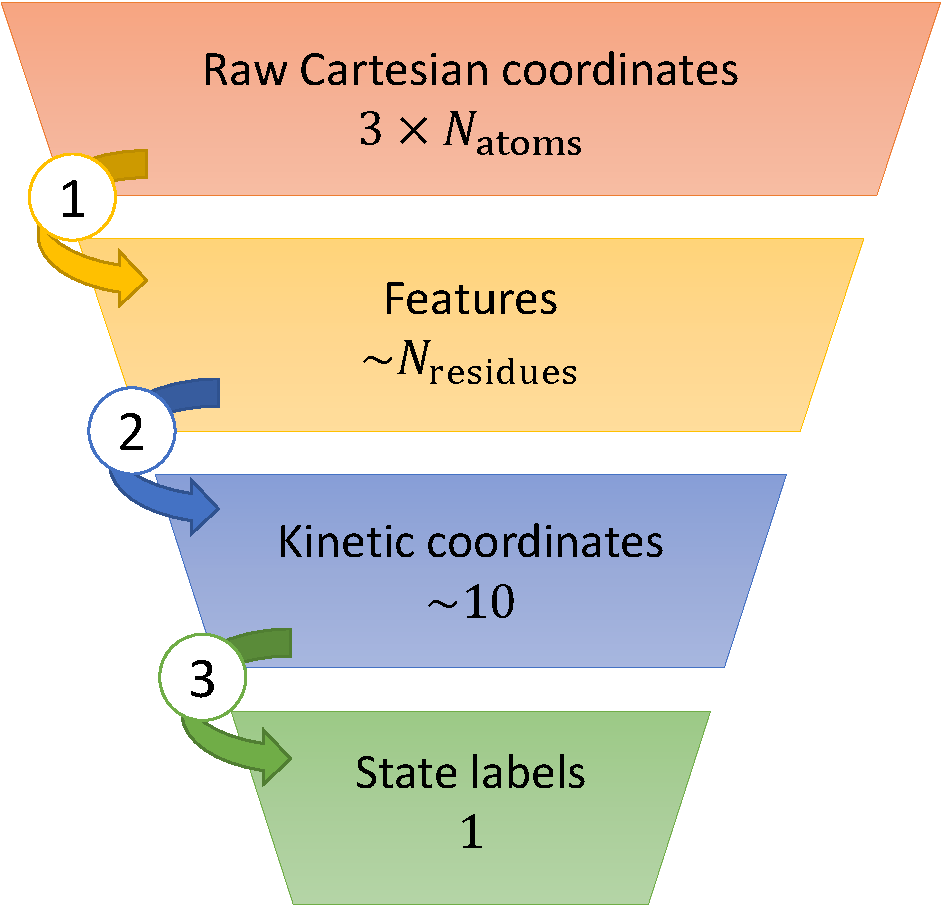
\includegraphics[width=0.9\linewidth]{1-src/dimreduce}
\caption{\textbf{Data transformations and their dimensionality.}
    Markov state models (MSMs) partition dynamical data into a set of
    states and estimate rates between them. A typical pipeline for state
    definition consists of a series of transformations (indexed by circled numbers)
    between representations of the data. Each step projects a higher
    dimensional representation onto a lower dimensional representation. The
    approximate dimension of each representation is reported below the
    representation name.
    Although not traditionally thought of as a 
    dimensionality reduction, clustering (step 3) 
    reduces each frame to a single integer cluster label.
}
\label{fig:dimreduce}
\end{figure}

\begin{figure}[htbp]
\centering
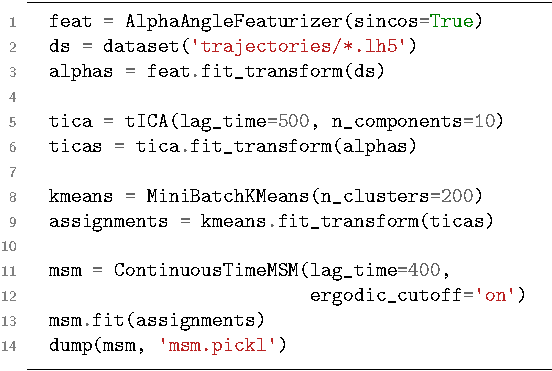
\includegraphics[width=\linewidth]{1-src/code}
\caption{\textbf{Sample MSM code.}
    MSMBuilder balances a powerful API (application programming interface) with ease of use.
    A sample workflow
    is shown here using the Python API. Following the successful model of
    the broadly-applicable \texttt{scikit-learn} package, each modelling step is
    represented by an estimator object which operates on the data. Here, the
    \texttt{AlphaAngleFeaturizer} transforms raw coordinates into
    $\alpha$ angles. The output of this transformation is fed into the
    \texttt{tICA} dimensionality reduction, \texttt{MiniBatchKMeans}
    clustering algorithm, and finally into the \texttt{ContinuousTimeMSM}
    model. MSMBuilder provides a litany of utility functions for dealing
    with large molecular dynamics datasets for I/O. While this example
    shows the Python API, MSMBuilder is fully functional from the command
    line with an intuitive 1-to-1 correspondence between Python estimator
    objects and command-line commands.
}
\label{fig:src-code}
\end{figure}

\begin{figure}[htbp]
\centering
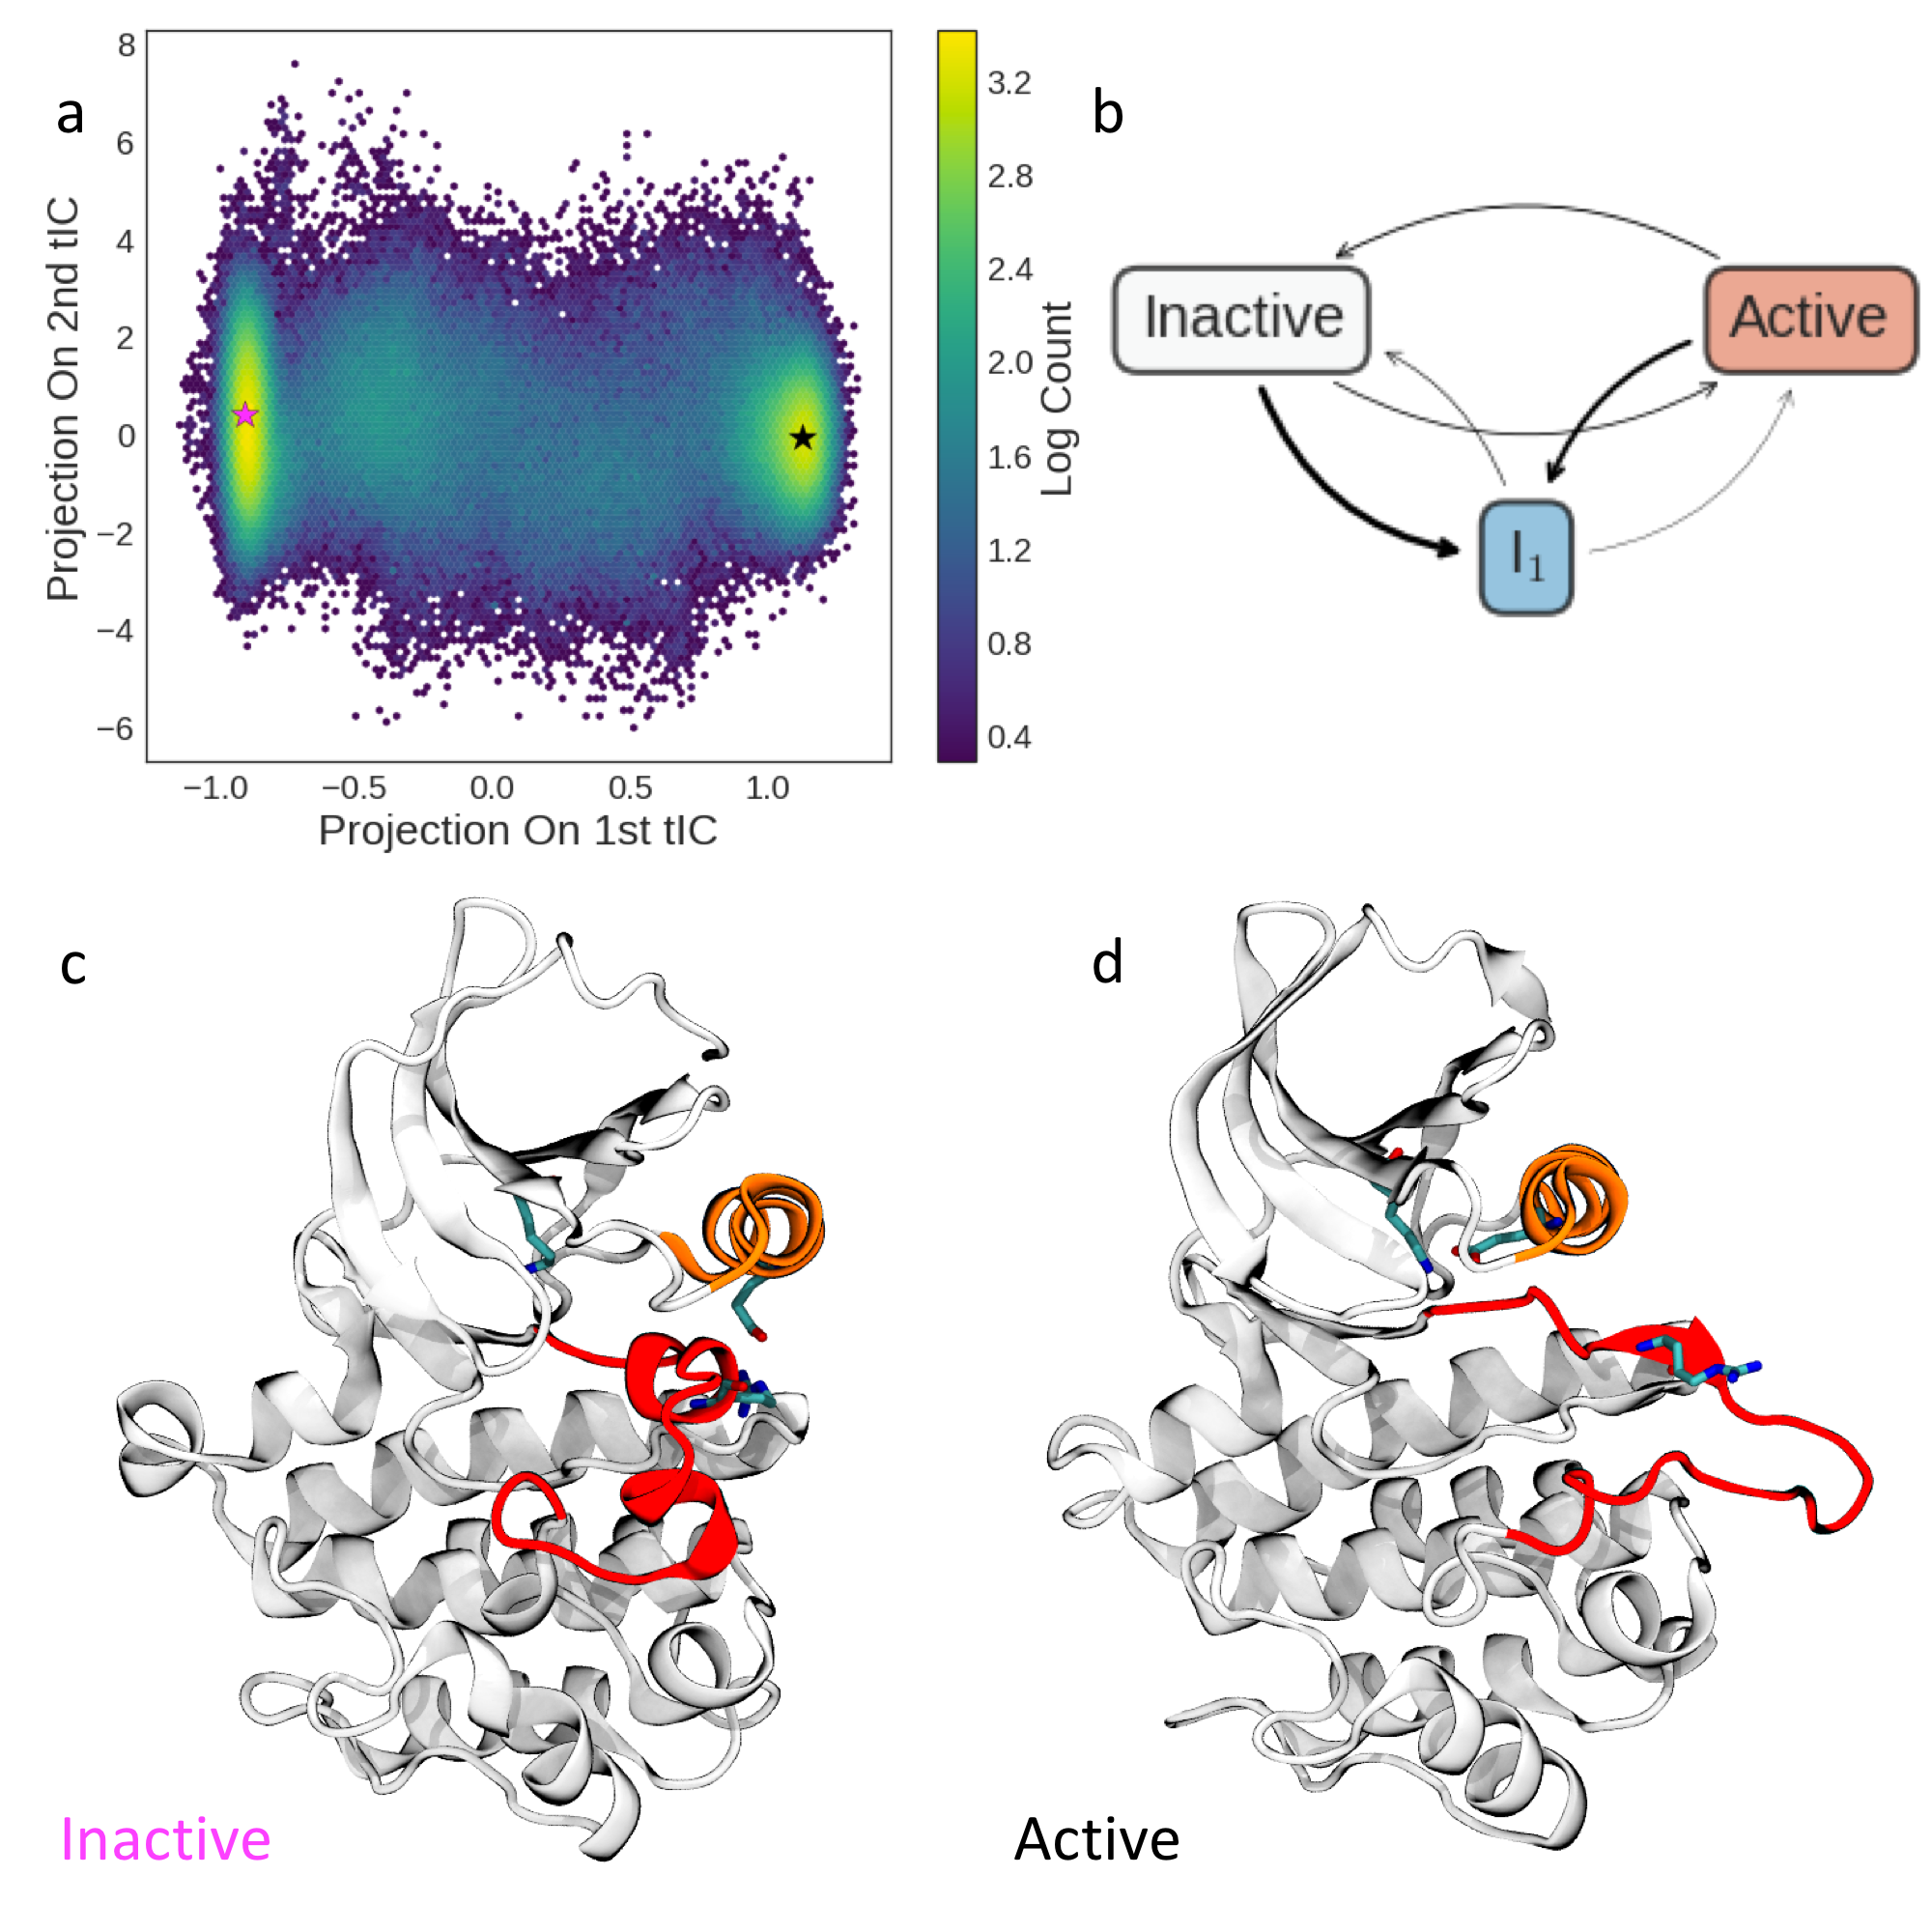
\includegraphics[width=\linewidth]{1-src/plot}
\caption{\textbf{c-Src kinase MSM.}
    MSMBuilder constructs interpretable models from large datasets.  This
    figure shows a 2D-histogram for the Src kinase from tICA-MSM analysis
    projected onto the dominant modes of a tICA model (a).  A simple
    macrostate model of the dynamics shows the presence of an intermediate
    state I$_1$ connecting the inactive and active states (b). The arrow
    thickness corresponds to the rate of transitions. The model
    indicates that the active state (red) is the most stable state followed
    by the inactive and intermediate states (gray and blue, resp.).
    The analysis discovers a coordinate (the first tIC) between the known
    active and inactive conformations. Representative structures
    are selected from MSM states and show the conformational differences
    between the two basins. The unfolding of the activation loop (red
    helix) forms a catalytically active Src capable of initiating and
    regulating downstream signaling pathways (c and d). 
}
\label{fig:src}
\end{figure}

MSMBuilder allows rapid analysis of large molecular dynamics datasets. In
this example, we construct an MSM of a kinase molecule.  Kinases are
critical enzymes that control cellular pathways. Malfunctions of kinases
have been linked to many different cancers
\cite{Taylor_TrendsBiochemSci11}.  Here, we use MSMBuilder to study the
c-Src kinase, a regulator of cellular growth \cite{Shukla_NatCommun14}, and
demonstrate that the resulting MSM can capture activation dynamics.
Understanding the activation process reveals atomistic, kinetic,
and thermodynamic insights into the protein's conformational
heterogeneity, which can help design better therapeutics.

Broadly, the procedure for constructing an MSM is to define a set of states
and then estimate transition rates among those states.  Before beginning
model construction, researchers must obtain time-series data they wish to
model.  Usually, this is the output of a molecular dynamics engine
(MSMBuilder supports nearly every MD trajectory file format \cite{2015-mdtraj}), 
but it
could also be experimental time-series measurements. For this example, we
use a previously-generated MD dataset of the c-Src kinase, publicly
available from the Stanford Digital Repository (SDR) \footnote{Available here:
https://goo.gl/LLchMT.  For simulation details, see
\citet{Shukla_NatCommun14}.}. 

The first step of model construction is to transform the raw Cartesian
coordinates into vector features that are invariant to
translation and rotation (\cref{fig:dimreduce}, step
1).  Here, we project our trajectory frames onto the dihedral angles
created by each set of four consecutive alpha carbons ($\alpha$ angles)
\cite{Flocco_ProteinSci95}.  This reduces the dimensionality of the data
from 12,693 Cartesian coordinates to 518 features.  The appropriate
featurization depends on the particular system under study (see \cref{sec:example-gmrq}). MSMBuilder
offers a collection of featurization strategies with a unified interface.
Popular features include backbone and side chain dihedrals (through the
\texttt{DihedralFeaturizer} class), heavy atom or  C$_\alpha$ contact
distances (\texttt{ContactFeaturizer}), distance of reciprocal inter-atomic
distances (\texttt{DRIDFeaturizer}) \cite{2012-drid}, and root mean squared
deviation to a set of structures (\texttt{RMSDFeaturizer}). There are
additional utilities for concatenation of multiple choices of features and
feature scaling.
% Note: ariana thinks that feature scaling needs more explanation
% I can't think of a way to describe it without messing up the flow of
% this section. Plus there is a wikipedia article named "feature scaling",
% so I don't think it's too unique a term.

The second step in MSM construction projects structural features onto
a lower-dimensional subspace
(\cref{fig:dimreduce}, step 2). This improves the statistical qualities
of subsequent steps, but may discard important information if the
projection is not carefully chosen.
Time-structure based independent
component analysis (tICA) finds a set of ``slow" (high autocorrelation)
coordinates. In practice, this dimensionality reduction
has proven to be very useful for capturing
slow, biophysical conformational change 
\cite{2013-schwantes-tica, 2013-noe-tica}.
In this example, we reduce the dimensionality
of our kinase data from 518 dihedrals to 5 tICA coordinates.
MSMBuilder includes support for similar algorithms
(\texttt{SparseTICA} \cite{2016-sparsetica}) as well as general manifold
learning algorithms like principal components analysis (\texttt{PCA}),
\texttt{SparsePCA}, or \texttt{MiniBatchSparsePCA}. Prior to 2013, this
step was not available for model construction. Accordingly, software
available at the time could not easily be extended to accomodate tICA
intermediate processing. The design of MSMBuilder~3 permits arbitrary
addition, subtraction, and re-ordering of data transformation steps.

Next, we define the states of our MSM by grouping conformations which
interconvert rapidly (\cref{fig:dimreduce}, step 3). For the c-Src kinase,
we employ the \texttt{MiniBatchKMeans} \cite{2010-minibatch-kmeans}
clustering algorithm to parition our data into 200 microstates. We note
that our data has been reduced from 5 tICA
coordinates to one integer cluster label per frame. 
The prior dimensionality reduction
permits using off-the-shelf clustering algorithms. Accordingly,
MSMBuilder supports K-Means like clustering algorithms (\texttt{KCenters},
\texttt{KMedoids}, and  \texttt{MiniBatchKMedoids}), and hierarchical clustering.

With our states defined, we proceed to estimate the rates among them. As
the final model construction step, we learn a continuous-time MSM
\cite{2015-ratematrix} from our labeled trajectories. We have chosen to use
a continuous-time MSM to directly estimate transition rates; we could have
alternatively built a traditional MSM (to estimate transition
probabilities) or a hidden Markov model (HMM). We direct interested readers
to a more thorough application of HMM modelling to the c-Src dataset
\cite{2014-hmm}. The relevant Python code for constructing this MSM is
shown in \cref{fig:src-code}. Complete, executable code is available in the
SI as an IPython \cite{2007-ipython} notebook.

To draw interpretable conclusions from our data via Markov modelling, we
query the model.  For c-Src, we use MSMBuilder to relate model behavior to
biological function.  We present a log-scaled 2D histogram
(\cref{fig:src}a) of the trajectories projected onto the two dominant slow
processes, or ``tICs'', from our tICA model. We then sample the centroids
of states (shown as pink and black stars) in low free energy regions to
visualize representative configurations in three dimensions \cite{1996-vmd}
(\cref{fig:src}c and d). The dominant tIC (x-axis) highly correlates with
the activation of the kinase. Kinase activation requires the unfolding of
the activation loop (red) and an inward swing of the catalytic helix
(C-helix). The inward rotation of the helix coincides with the switching of
hydrogen bonding pair from Glu-Arg  to Glu-Lys (licorice). We investigate
the dynamics between the active, inactive, and intermediate macrostates by
applying Robust Perron Clustering Analysis (PCCA+) to our MSM. PCCA+ is a
spectral clustering method, which lumps MSM states into an arbitrary number
of metastable macrostates, facilitating qualitative analysis of rates and
populations among biologically-relevant macrostates \cite{2005-pcca}. The
rates among three macrostates are shown by the thickness of arrows in
\cref{fig:src}b. Further options of querying the model (not shown here but
available in MSMBuilder) include computation of relaxation timescales,
transition path theory analysis \cite{Metzner_MMS09, Berezhkovskii_JCP09,
Noe_PNAS09}, and generation of synthetic trajectories for visual
inspection.

The assortment of modeling options such as the choice of featurizer, the
use of dimensionality reduction, and the selection of the clustering
algorithm, along with any associated internal parameter choices, presents
the modeler with a motley of modeling decisions and tunable parameters.
In the next
section, we show how a scoring metric for MSMs can provide the modeler with
a unbiased protocol for determining which parameters are suitable given a
set of MD trajectories.

% vim: tw=75
